\documentclass{chi-ext}
% Please be sure that you have the dependencies (i.e., additional LaTeX packages) to compile this example.
% See http://personales.upv.es/luileito/chiext/

%% EXAMPLE BEGIN -- HOW TO OVERRIDE THE DEFAULT COPYRIGHT STRIP -- (July 22, 2013 - Paul Baumann)
\copyrightinfo{Permission to make digital or hard copies of all or part of this work for personal or classroom use is granted without fee provided that copies are not made or distributed for profit or commercial advantage and that copies bear this notice and the full citation on the first page. Copyrights for components of this work owned by others than ACM must be honored. Abstracting with credit is permitted. To copy otherwise, or republish, to post on servers or to redistribute to lists, requires prior specific permission and/or a fee. Request permissions from permissions@acm.org. \\
 {\emph{CHI'14}}, April 26--May 1, 2014, Toronto, Canada. \\
 Copyright \copyright~2014 ACM ISBN/14/04...\$15.00.}
% DOI string from ACM form confirmation}
%% EXAMPLE END -- HOW TO OVERRIDE THE DEFAULT COPYRIGHT STRIP -- (July 22, 2013 - Paul Baumann)

%\title{CHI \LaTeX\ Ext. Abstracts Template}
\title{Mute Robot - Cooperative Gameplay through Body Language Communication}

\numberofauthors{4}
% Notice how author names are alternately typesetted to appear ordered in 2-column format;
% i.e., the first 4 autors on the first column and the other 4 auhors on the second column.
% Actually, it's up to you to strictly adhere to this author notation.
\author{
  \alignauthor{
  	\textbf{Chun-Yen Hsu}\\
  	\affaddr{Department of Computer Science and Information Engineering}\\
  	\affaddr{National Taiwan University, Taipei, Taiwan}\\
  	%\affaddr{Authortown, PA 54321 USA}\\
  	\email{hcythomas0125@gmail.com}
  }\alignauthor{
  	\textbf{Han-Yu Wang}\\
  	\affaddr{Department of Networking and Multimedia}\\
  	\affaddr{National Taiwan University, Taipei, Taiwan}\\
  	%\affaddr{Authortown, PA 54321 USA}\\
  	\email{huw12313212@gmail.com}
  }
  \vfil
  \alignauthor{
  	\textbf{Ying-Chao Tung}\\
  	\affaddr{Department of Computer Science and Information Engineering}\\
  	\affaddr{National Taiwan University, Taipei, Taiwan}\\
  	%\affaddr{Authortown, PA 54321 USA}\\
  	\email{tony61507@gmail.com}
  }%\alignauthor{
  	%\textbf{Fifth Author}\\
  	%\affaddr{AuthorCo, Inc.}\\
  	%\affaddr{123 Author Ave.}\\
  	%\affaddr{Authortown, PA 54321 USA}\\
  	%\email{author6@anotherco.com}
  %}
  \vfil
  \alignauthor{
  	\textbf{Wei-Han Wang}\\
  	\affaddr{Department of Networking and Multimedia}\\
  	\affaddr{National Taiwan University, Taipei, Taiwan}\\
  	%\affaddr{Authortown, PA 54321 USA}\\
  	\email{wangweihang5566@gmail.com}
  }%\alignauthor{
  	%\textbf{Sixth Author}\\
  	%\affaddr{AuthorCo, Inc.}\\
  	%\affaddr{123 Author Ave.}\\
  	%\affaddr{Authortown, PA 54321 USA}\\
  	%\email{author7@anotherco.com}
  %}
}

% Paper metadata (use plain text, for PDF inclusion and later re-using, if desired)
\def\plaintitle{CHI LaTeX Extended Abstracts Template}
\def\plainauthor{Luis A. Leiva}
\def\plainkeywords{Game; Video games; Game design; Body language; Kinect}
\def\plaingeneralterms{Documentation, Standardization}

\hypersetup{
  % Your metadata go here
  pdftitle={\plaintitle},
  pdfauthor={\plainauthor},  
  pdfkeywords={\plainkeywords},
  pdfsubject={\plaingeneralterms},
  % Quick access to color overriding:
  %citecolor=black,
  %linkcolor=black,
  %menucolor=black,
  %urlcolor=black,
}

\usepackage{graphicx}   % for EPS use the graphics package instead
\usepackage{balance}    % useful for balancing the last columns
\usepackage{bibspacing} % save vertical space in references


\begin{document}

\maketitle

\begin{abstract}
Speech ability, a general habit becoming nature for us, plays an important role in our daily life. Besides speech, using body language is an evident and feasible way to communicate between two people.
Mute Robot Game has been designed to provide players with a series of puzzle challenges where they both become robots without speech ability.
We encourage players to communicate with body language, with an emphasis on cooperation to facilitate immersion with each other.
In our user study, all participants thought it was interesting to communicate with body language and two-thirds of the players reported they could understand the other player’s body language.
%Players need to cooperate with each other to pass challenges by using body language communication.
\end{abstract}

%\begin{abstract}
%In this sample we describe the formatting requirements for various %SIGCHI related submissions 
%and offer recommendations on writing for the worldwide SIGCHI %readership. 
%%Do not change the page size or page settings.
%Please review this document even if you have submitted to SIGCHI %conferences before, 
%some format details have changed relative to previous years.
%\end{abstract}

%[Section] Author Keywords
\keywords{\plainkeywords}
%\textcolor{red}{Mandatory section to be included in your final version.}

%[Section] ACM Classification Keywords
\category{K.8.0}{Personal Computing}{General \it{Games}}. 
%See \cite{ACMCCS} 
%See: \url{http://www.acm.org/about/class/1998/} 
%for help using the ACM Classification system.
%\textcolor{red}{Mandatory section to be included in your final version.}

%[Section] General Terms
%\terms{\plaingeneralterms}
%\textcolor{red}{Optional section to be included in your final version.}

% =============================================================================
\section{Introduction}
% =============================================================================
Using body langauge to communicate with people from different regions or speaking different languages is a common solution. 
Therefore, we try to construct a creative gameplay to immerse this communication way in the reality to a virtual world.
It is a cross-language game for human beings around the world. 
This idea is somewhat influenced by Ways\cite{Ways}. Although Ways proposed a similar gameplay in 2011, they still used keyboards and mouses as input devices.
Because of the restriction of controlling avatars in Ways by keyboards and mouses, we provides Mute Robot, a novel game combining kinect to capture players postures and then precisely apply them to avatars in the game.
Mute Robot is a cooperative platformer with two players connected over the internet.
By corresponding players' motions to avatars in the game, Mute Robot attempts to create an innovative gameplay of letting players communicate with each other only using body language.


Without any other ways of communication, players need to operate on the same wavelength or build their own connection pattern by body language at the beginning.
After finishing building their own connection between each other, players start to solve a serial of puzzles with their own communication pattern.
For example, in the first level, there is a door locked on the right side, players have to tread three buttons on the ground with the correct sequence to unlock the door.(fig. 2)
However, only the upper side player know the sequence, the underside player can trample those buttons, so they need to pass the right pattern with the communication method they built before.

The focus in Mute Robot lies on this cross-language desgin for the core gameplay.
In order to make all players experience both acting an information sender and a receiver, we switch password stages between the upper side and the down side at different levels.
Morevoer, Mute Robot desires to explore the limitation of communicating without normal methods , so the game require the password sender acting more and more difficult objects with body language.
For example, in the second stage, there are a circle and a x on the first wheel and then three numbers on the second one. It increases the difficulty on the communication between the two players.(fig. 1)
Thus, players need to evaluate their own connection modus stronger and stronger to deal with the increasing difficulty in the game. 

 
  
% =============================================================================
\section{Design and Development}
% =============================================================================
Mute Robot is a cooperative puzzle platformer game using Unity3D\cite{Unity3D} engine. The game involves two players connected over Internet. During the game play, two players are physically separated in different rooms. 
They cannot talk to each other directly and the only way to communicate is using their body language. 
In each room, we provide a wii\cite{Wii} controller and a Kinect\cite{Kinect} device. 
The wii controller is used to control the avator movement, like jump or move. 
In the mean time, Kinect is applying the player's body language to his own avatar. 

%why use wii, why not use pure Kinect control!?

\begin{figure}
  \centering
  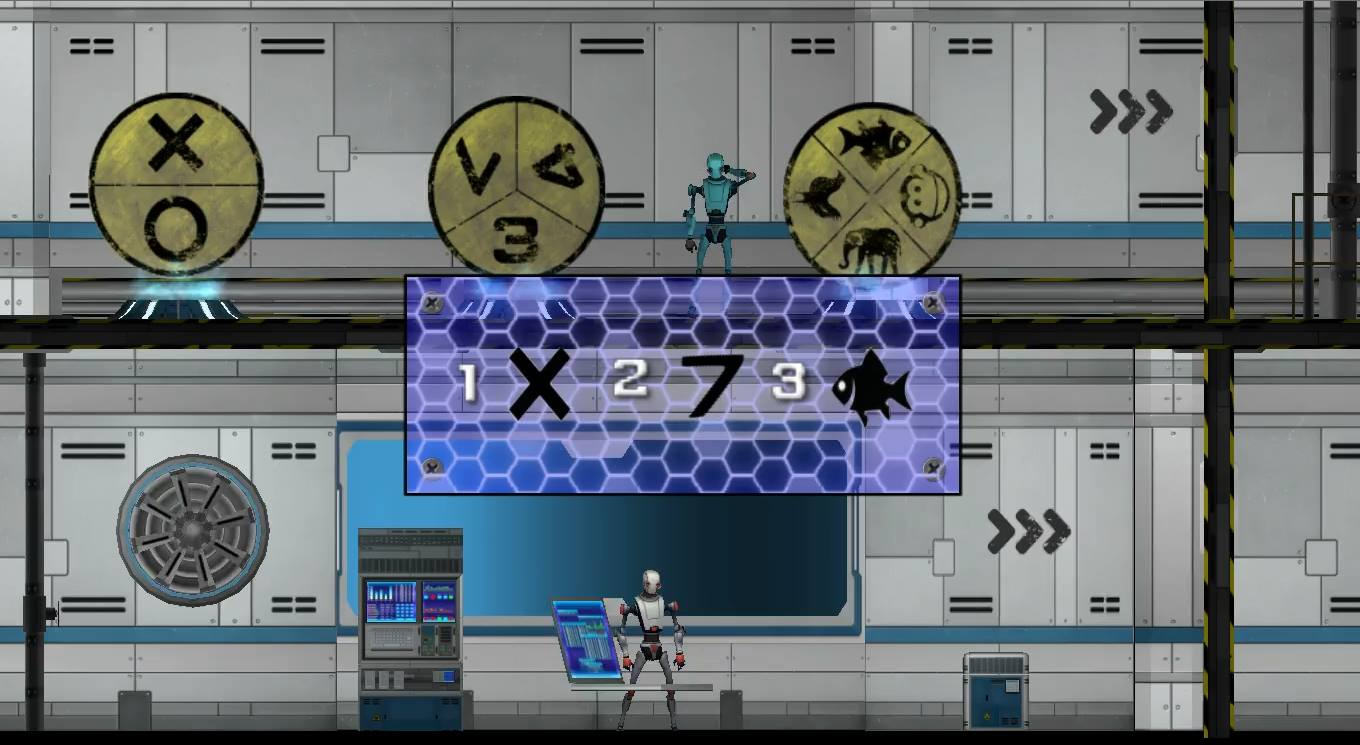
\includegraphics[width=\linewidth]{figures/Figure1.jpg}
  \caption{The asymmetric puzzle system from Mute Robot.}
  \label{fig:Figure1}
\end{figure}


\section{Using Body Language}
% =============================================================================
%關卡設計方式
%In order to apply a new communication interface for user, Mute Robot is designed by using body language to communicate between players. Testing shows that using body language is an intuitive choice for player to communicate without speech ability.

To encourage players using body language, we design an asymmetric puzzle system. Only one player can receive puzzle hints, and the other player can solve the puzzle afterwards.
Taking one of our game stage for example(fig. 1), there is a locked door on the right side which obstructs both players' route to the next stage. 
%With a view to opening the locked door, the underside player will receive some puzzle-solving message. 
The upper side player can't see the puzzle-solving hints but he can turn the wheel to the match puzzle answer, which opens the locked door.
The only way to pass the stage is that the underside player needs to pass the puzzle-solving message to the other player with body language. 
%As a result, the right side locked door will be opened when all wheels are turned to the correct direction.

%If human beings lose speech ability, with no doubt, an intuition way for people communication is using body language. Based on past historical experience, using body language is a human instinct. In addition,  We assume that 

% =============================================================================
\section{Testing and Evaluation}
% =============================================================================

\marginpar{
\begin{figure}
  \centering
  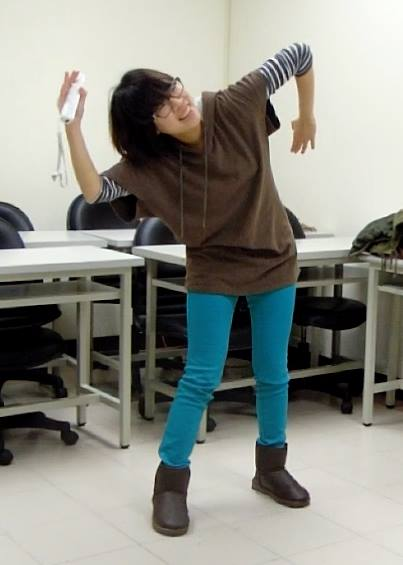
\includegraphics[width=0.8\linewidth]{figures/Figure3.jpg}
  \caption{A player performs pictogram (letter ``N'') with body language.}
  \label{fig:Figure3}
\end{figure}
}

We recruited 16 participants, and randomly divided them into 8 groups. In each group, participants did not know each other. We captured the players' movement through camera and the gameplay was also screen-recorded by Fraps\cite{Fraps}.
On average, the total game duration was about 10 to 20 minutes. 
At the end of the game, we provided a five-point Likert scales questionnaire to 
collect players' feedback for any possible improvement to gameplay experience.
%investigate the gameplay experience and collect player feedback.

\begin{figure}
  \centering
  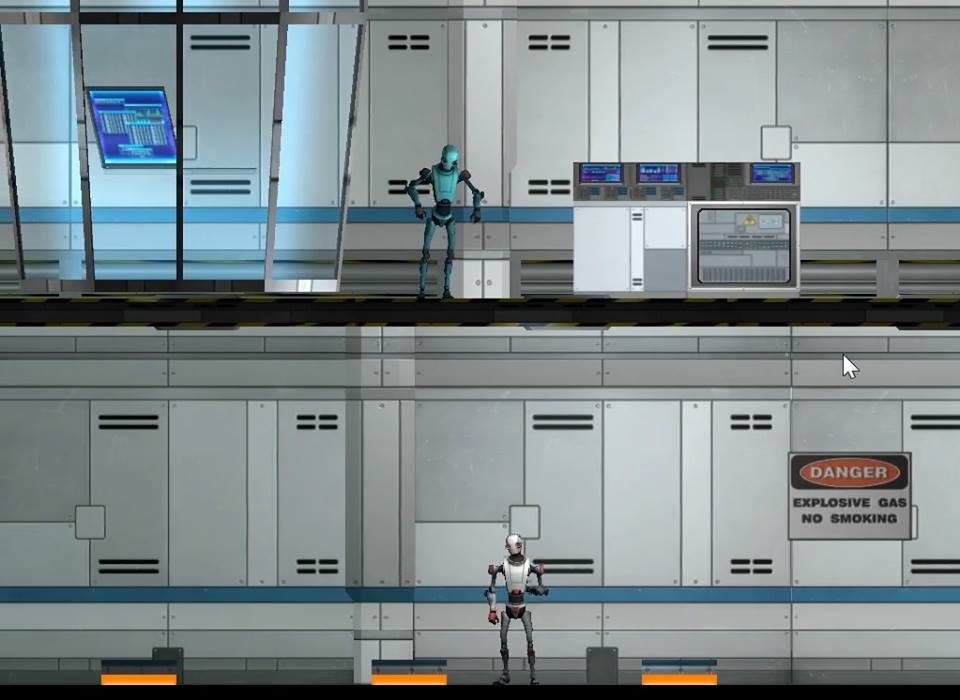
\includegraphics[width=0.8\linewidth]{figures/Figure2.jpg}
  \caption{A puzzle from Mute Robot, the upper side player knows the puzzle-solving sequence and passes the hint to the underside player.}
  \label{fig:Figure2}
\end{figure}

According to the video we recorded, we found out some unique strategies between players' body language communication: 
(1) {\bf Command style}: player who received puzzle-solving hints would command the other player to do some action directly. For instance, the player would wave his hand to tell the other player to go back; or the player liked to jump in place in order to imply the other player to tread on the relative position.
(2) {\bf Repeat after me}: player who received puzzle-solving hints would do the puzzle-solving actions one time for the other player to observe and emulate. For example, one of our game stage needed to open the locked door by jumping on three buttons respectively with a specific order(fig. 3). The upper side player might perform the answer all at once for the underside player to repeat.
(3) {\bf Pictogram style}: player would use his own body to express what he saw from puzzle-solving hints. As in figure 2, one participant wanted to express the letter ``N'' to the other player. Her solution was using her body to perform pictogram to show the character.


\begin{figure}
  \centering
  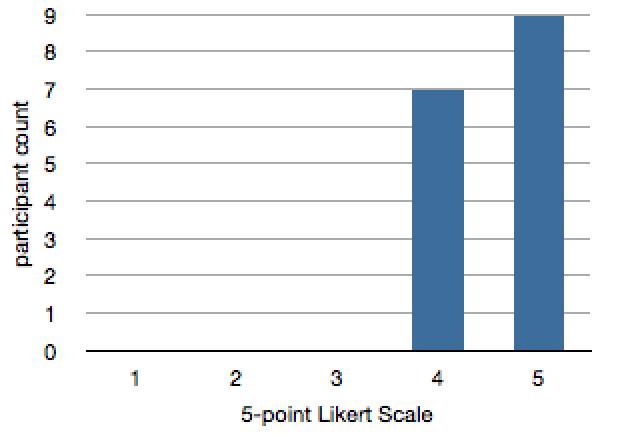
\includegraphics[width=0.8\linewidth]{figures/1_BLisInteresting.png}
  \caption{Interesting level of using body language.}
  \label{fig:1_BLisInteresting}
\end{figure}

The results from the questionnaires could support our Mute Robot game design. 
Figure 4 shows that all participants thought it is interesting to use body language to communicate in puzzle game.
%有趣,了解對方的語言、有好感
Figure 5 shows that about two-thirds of the players reported they could understand the other player's body language.


\begin{figure}
  \centering
  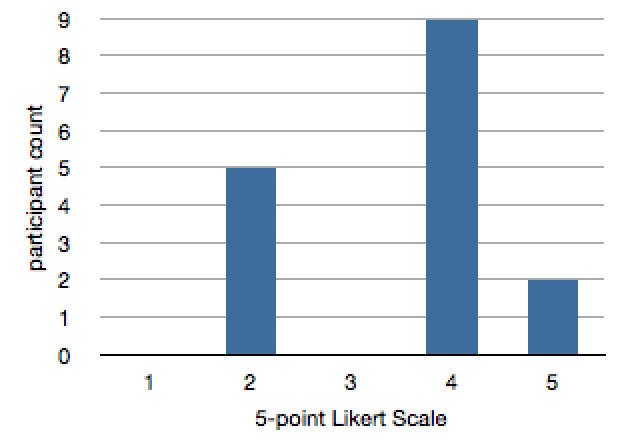
\includegraphics[width=0.9\linewidth]{figures/2_BLunderstand.png}
  \caption{Understanding level of the teammate's body language.}
  \label{fig:2_BLunderstand}
\end{figure}

%\begin{figure}
%  \centering
%  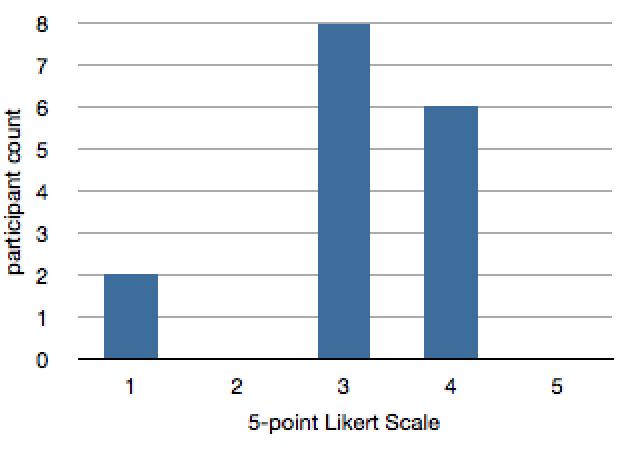
\includegraphics[width=0.8\linewidth]{figures/3_BLPositiveFeeling.png}
%  \caption{333}
%  \label{fig:3_BLPositiveFeeling}
%\end{figure}

%situations
%1. 命令句:如果畫面鐘有那個東西,會直接用指的, 回來手勢,
%2. 做給他看(踩左右中)
%3. 象行(angry中的N), 模仿動物 directly

%找16位玩家,不認識對方
%遊戲長度約10~20分鐘
%- # 
%- Body Language Communication (observation)
%- Satisaction Survey



% =============================================================================
\section{Future Work}
% =============================================================================

Currently, our system only tracks significant body movement, which leaves behind important contexts in facial expression and finger movements. As far as we are concerned, with these detailed information, we can communicate with body language more precisely. For example, in the face of number expression, player can intuitively use his fingers to show the number. On the other hand, facial detail can express players' emotion directly that help players know his teammate's feeling and connect two players more deeply.
%加例子!
%有手指跟表情,溝通更容易&直觀

%We believe with these detailed information, we can communicate with body language more precisely. 
%Kinect allows personal computer to track the gesture of our body as we move around, but it hasn't had the fine detail of our gestures, and particular, it hasn't really understood our hand. If one day, the ability for Kinect can recognize our hand gesture and facial expression, we can communicate with body language more precisely. 

Futhermore, Mute Robot game design is using asymmetric puzzle system to let players cooperate with each other. In other words, it only requires one-way message passing.
%one way
%若有雙向溝通感情會更好,因兩人的參與度可以提升 or 成就感可以便高(都有做到事情....)
In the future, we encourage to appear more two-way message passing between players. 
If both players can receive part of puzzle-solving hints and exchange messages with body language, we believe that it will have more deeply interaction between players and become more interesting.

%1. 可以抓到表情、手指
%2. 可以做更複雜的關卡
%now:一個人告訴另一個人,不是兩邊整合訊息 (a告訴b
%improve:上下皆有一些資料,共同完成 a purpose

% =============================================================================
\section{Conclusion}
% =============================================================================
Mute Robot shows a new integration between current cooperative gameplay and body language
%加合作
%The Kinect-based 
, and our design can facilitate the body language interaction and intrinsically motivate the player.
The interaction between game and human body movement form an unprecedented innovative gameplay empiriment.
%Mute Robot can proliferate cooperation and interaction between players.
Our user study results also indicate that body language based cooperative gameplay is practical and entertaining.
%加一句真正可以做什麼
Mute Robot provides a path towards future exploration of this relatively unexplored field of game design with capacious development space.

%數據 feadback 喜歡 
%這樣的作法、遊戲是蠻有發展空間的
%是一個很適合在kinect上的發展遊戲


\section{Acknowledgements}
We thank advisor Mike Y. Chen and the faculty and staff of National Taiwan University.
We would also like to express our gratitude towards all playtesters who have helped us in our many iterations. 


%\section{References format}
%References must be the same font size as other body text.
% REFERENCES FORMAT
% References must be the same font size as other body text.

\balance
\bibliographystyle{acm-sigchi}
\bibliography{chi14SGC-MuteRobot}

\end{document}